\documentclass{article}

\usepackage{amsmath}
\usepackage[usenames,dvipsnames]{color}
\usepackage{multirow}
\usepackage{listings}
\usepackage[a4paper, top=2cm, bottom=3cm, left=2cm, right=2cm]{geometry}

\usepackage{tikz}
\usetikzlibrary{arrows,shapes,shapes.multipart,shapes.geometric,
	snakes,automata,backgrounds,petri,calc}
\usetikzlibrary{positioning}

\newcommand{\bfc}{{\sc Bfc}}
\newcommand{\mist}{{\sc Mist}}
\newcommand{\pnerf}{{\sc Pnerf}}
\newcommand{\zthree}{{\sc Z3}}
\newcommand{\ttt}[1]{\texttt{#1}}
 
\tikzstyle{place}=[circle,thick,draw=black!75,fill=white!20,
  	minimum size=6mm]
\tikzstyle{red place}=[place,draw=red!75,fill=red!20]
\tikzstyle{blue place}=[place,draw=blue!75,fill=blue!20]
\tikzstyle{transition}=[rectangle,thick,draw=black!75,
  	fill=black!20,minimum size=4mm]

\tikzstyle{state}=[draw, ellipse, aspect=2]
\tikzstyle{action}=[draw, rectangle, align=center]
\tikzstyle{decision}=[draw, diamond, aspect=2, align=center]
\tikzstyle{print}=[draw, trapezium, trapezium left angle=70, trapezium right angle=-70]
\tikzstyle{every edge}=[draw, ->, >=stealth, shorten >=2pt, shorten <=2pt]

\begin{document}

\title{Report on a Safety Checker for Petri nets}
\author{Philipp Meyer \and Rusl\'{a}n Ledesma-Garza}
% \institute{Technische Universit\"at M\"unchen}
\date{Wed Nov 13 09:11:15 CEST 2013}



\section{Preliminaries}


\begin{verbatim}
* Petri net:
 N = (S, T, E, M0), where
 S : places
 T : transitions
 E : edges
 M0: initial marking

* Property:
 P, linear arithmetic formula
\end{verbatim}
\iffalse
\begin{verbatim}
 Examples:
  x + y < 0
  x + y < 0 \\and x + z > 0
  x + y < 0 \\or  x + z > 0

 ~P = (x + y <  0 \\and x + z >  0) \\or  x + z >  0
  P = (x + y >= 0 \\or  x + z <= 0) \\and x + z <= 0
\end{verbatim}
\fi

\newpage
\section{Method Safety}

The method Safety checks that a given Petri net \verb=N= never violates a property \verb=P=.
We present the method Safety by example on a simplified mutual exlusion algorithm by Delzanno2001.

\begin{verbatim}
* Code

bool m = false;

// Thread 1:
while (true) {
  if (! test_and_set(m)) {
    // critical section 1
    m = false
  }
  if (! test_and_set(m)) {
    // critical section 2
    m = false
  }
}

// Thread 2:
while (true) {
  if (! test_and_set(m)) {
    // critical section 1
    m = false
  }
  if (! test_and_set(m)) {
    // critical section 2
    m = false
  }
}

* Property: Thread 1 and Thread 2 are never in any critical section at the same time.

* Petri net

Place m is marked in the net exactly if m is false in the algorithm.

\end{verbatim}

\begin{center}
  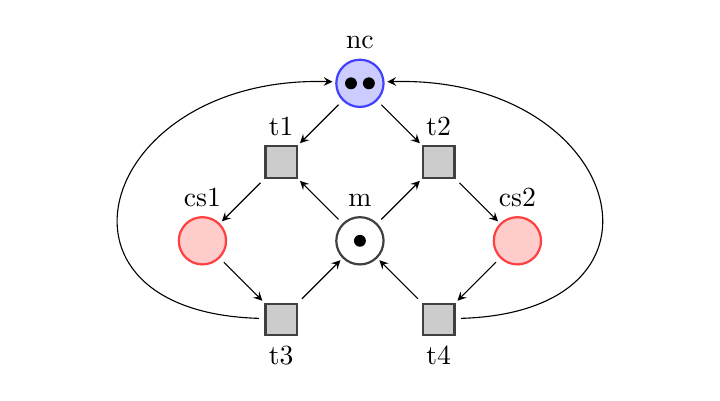
\begin{tikzpicture}[node distance=2cm]
    \node[blue place, tokens=2, label=above:nc] (nc) {};
    \node[place, tokens=1, label=above:m, below of=nc] (s) {};
    \node[red place, label=above:cs1, left of=s] (cs1) {};
    \node[red place, label=above:cs2, right of=s] (cs2) {};
    \node[transition, label=above:t1] (t1) at ($(s)!0.5!(cs1) + (0,1cm)$) {}
    edge [pre] (nc)
    edge [pre] (s)
    edge [post] (cs1);
    \node[transition, label=above:t2] (t2) at ($(s)!0.5!(cs2) + (0,1cm)$) {}
    edge [pre] (nc)
    edge [pre] (s)
    edge [post] (cs2);
    \node[transition, label=below:t3] (t3) at ($(s)!0.5!(cs1) - (0,1cm)$) {}
    edge [pre] (cs1)
    edge [post] (s)
    edge [post,bend left,min distance=3cm, out=105, in=105] (nc);
    \node[transition, label=below:t4] (t4) at ($(s)!0.5!(cs2) - (0,1cm)$) {}
    edge [pre] (cs2)
    edge [post] (s)
    edge [post,bend right,min distance=3cm, out=-105, in=-105] (nc);
  \end{tikzpicture}
\end{center}

\begin{verbatim}
* Property: P = ( cs1 + cs2 <= 1 )
\end{verbatim}

\newpage
\begin{verbatim}
* Method Safety:

  Subprocedure \mathcal{C} constructs state constraints C corresponding to N.
\end{verbatim}

\begin{center}
  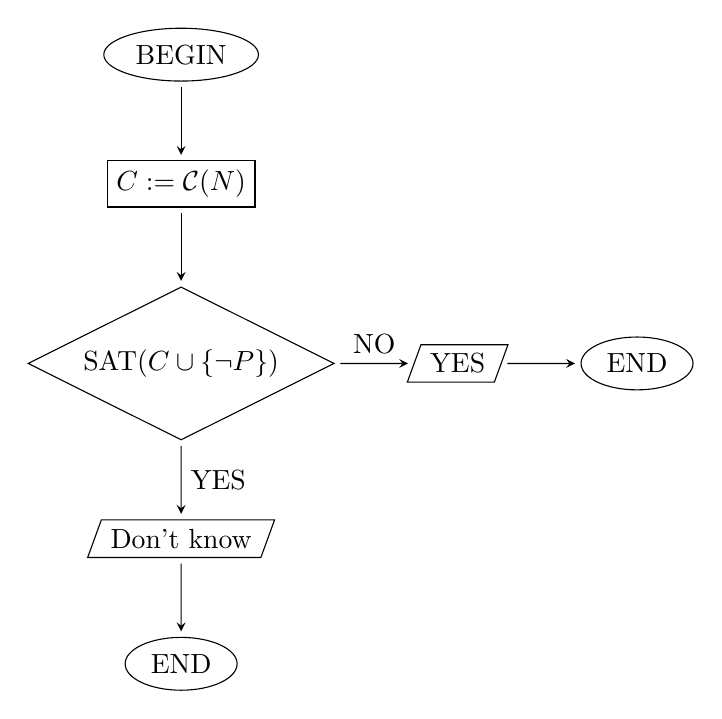
\begin{tikzpicture}
    \node[state] (begin) {BEGIN};
    \node[action, below=of begin] (c) {$C:=\mathcal C(N)$};
    \node[decision, below=of c] (satc) {$\text{SAT}(C \cup \{\neg P\})$};
    \node[print, right=of satc] (yes) {YES};
    \node[print, below=of satc] (dontknow) {Don't know};
    \node[state, right=of yes] (end1) {END};
    \node[state, below=of dontknow] (end2) {END};
    
    \draw (begin) edge (c);
    \draw (c) edge (satc);
    \draw (satc) edge node[above]{NO} (yes);
    \draw (yes) edge (end1);
    \draw (satc) edge node[right]{YES} (dontknow);
    \draw (dontknow) edge (end2);
  \end{tikzpicture}
\end{center}

\begin{verbatim}
* Property of state constraints C: if C U {\neg P} is unsat then N |= P

* State constraints C:

  Place equations:

  nc      = 2 - t1 - t2 + t3 + t4
  ^         ^   ^    ^    ^    ^
  |         |   |    |    |    |
  place nc  |   ------    ------
            |      |         |
            |      |       input transitions of nc
            |      |    
            |    output transitions of nc
            |
         initial number of tokens in nc

  m     = 1 - t1 - t2 + t3 + t4
  cs1   = 0 + t1 - t3
  cs2   = 0 + t2 - t4

  Non-negativity conditions:

  nc  >= 0
  m   >= 0
  cs1 >= 0
  cs2 >= 0
  t1  >= 0
  t2  >= 0
  t3  >= 0
  t4  >= 0
\end{verbatim}

\newpage
\begin{verbatim}
* Place equation:
  
  For a given place s the place equation is

  s = initial number of tokens of place s - output transitions of s + input transitions of s

* Non-negativity conditions:

  place      >= 0
  transition >= 0

* Subprocedure \mathcal{C}:

  Input:
    (S, T, E, I) : Petri net
  Output:
    C : State constraints

  TODO: Unroll pseudocode?
\end{verbatim}

\newpage
\section{Method Invariant}

Given Petri net \verb?N? that does not violate property \verb?P?, method Invariant constructs an invariant \verb?I? with the following properties.
\begin{itemize}
\item For each reachable marking \verb=M=, \verb?I(M)? is valid.
\item For markings that violate the property, \verb?I(M)? is unsat.
\item \verb?I? is inductive:
  \verb?\forall M. I(M) valid ^ M -> M1 implies I(M1) valid?
\end{itemize}

\begin{verbatim}
* Code, property, and Petri net: same as in section Method Safety.
\end{verbatim}

\begin{verbatim}
* Method Invariant

  Subprocedure \mathcal{C'} constructs dual state constraints C' corresponding to N and P.
  Subprocedure Model returns assignment A such that A satisfies C'.
  Subprocedure Inv constructs invariant I corresponding to N, P, and A.
\end{verbatim}

\begin{center}
  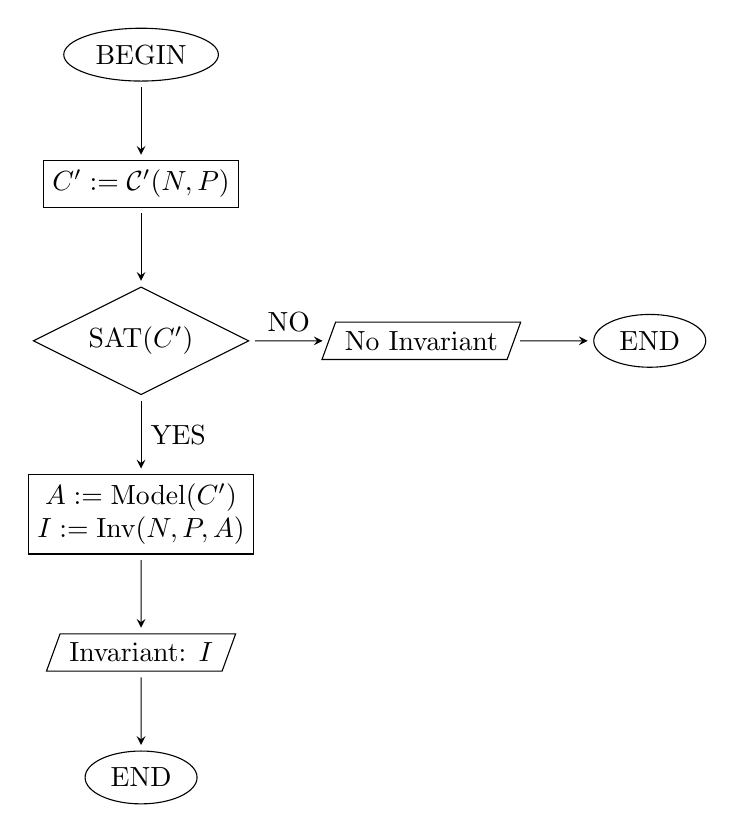
\begin{tikzpicture}
    \node[state] (begin) {BEGIN};
    \node[action, below=of begin] (c) {$C':=\mathcal C'(N, P)$};
    \node[decision, below=of c] (satc) {$\text{SAT}(C')$};
    \node[print, right=of satc] (noinv) {No Invariant};
    \node[action, below=of satc] (inv) {$A:=\text{Model}(C')$\\
      $I := \text{Inv}(N, P, A)$};
    \node[print, below=of inv] (printinv) {Invariant: $I$};
    \node[state, right=of noinv] (end1) {END};
    \node[state, below=of printinv] (end2) {END};
    
    \draw (begin) edge (c);
    \draw (c) edge (satc);
    \draw (satc) edge node[above]{NO} (noinv);
    \draw (satc) edge node[right]{YES} (inv);
    \draw (noinv) edge (end1);
    \draw (inv) edge (printinv);
    \draw (printinv) edge (end2);
  \end{tikzpicture}
\end{center}

\newpage
\begin{verbatim}
* Dual state constraints C':

  - nc - m + cs1 <= 0
  - nc - m + cs2 <= 0
    nc + m - cs1 <= 0
    nc + m - cs2 <= 0

  2 \cdot nc + m < 2 \cdot target1

  Non-negativity conditions:

  target1 >= 0
  nc      >= 0
  m       >= 0
  cs1     >= target1
  cs2     >= target1
\end{verbatim}

\begin{verbatim}
* Model A:

  target1 = 1
  nc      = 0
  m       = 1
  cs1     = 0
  cs2     = 0
  
* Invariant:

  cs1 + cs2 + m <= 1

* Subprocedure \mathcal{C'}:

  Input:
    (S, T, E, I) : Petri net
    P            : Property
  Output:
    C'           : Dual state constraints


Input:
 N = (S, T, E, I)
   = ( (nc m cs1 cs2) (t1 t2 t3 t4) (e1 ... en) (2 1 0 0) )
 P = ( cs1 + cs2 <= 1 )

Intermediate results:

Create variable p for property P.

For t1 construct inequation `- nc - m + cs1 <= 0` in the following way.
   - input_places + output_places <= 0

For t2 construct inequation `- nc - m + cs2 <= 0` in the following way.
   - input_places + output_places <= 0

For t3 construct inequation `nc + m - cs1 <= 0` in the following way.
   - input_places + output_places <= 0

For t4 construct inequation `nc + m - cs2 <= 0` in the following way.
   - input_places + output_places <= 0

Output:
  - nc - m + cs1   <= 0
  - nc - m + cs2   <= 0
  + nc + m - cs1 <= 0
  + nc + m - cs2 <= 0

  2 \cdot nc + m < 2 \cdot target1

  Non-negativity conditions:

  target1 >= 0
  nc      >= 0
  m       >= 0
  cs1     >= target1
  cs2     >= target1

  

* Subprocedure Inv:


* Theorem Dual State Constraints: 

  TODO: Unroll ?
\end{verbatim}

\newpage

\iffalse
Constraints $\mathcal C'(N, P)$ with
$Y_1 = \begin{pmatrix}target1 \end{pmatrix}$,
$Y_2 =\begin{pmatrix}nc & m & cs1 & cs2\end{pmatrix}$,
$A =\begin{pmatrix}0 & 0 & 1 & 1 \end{pmatrix}$ and
$b =\begin{pmatrix}2 \end{pmatrix}$:

\begin{align*}
  target1 - nc - m + cs1 \le& 0 \\ 
  target1 - nc - m + cs2 \le& 0 \\ 
  - target1 + nc + m - cs1 \le& 0 \\ 
  - target1 + nc + m - cs2 \le& 0 \\ 
2 \cdot nc + m <& 2 \cdot target1 \\
  target1 \ge& 0 \\
  nc \ge& 0 \\
  m \ge& 0 \\
  cs1 \ge& 0 \\
  cs2 \ge& 0
\end{align*}

Satisfying assignment is $Y_1 = \begin{pmatrix} 1 \end{pmatrix}$ and
$Y_2 = \begin{pmatrix}0 & 1 & 0 & 0 \end{pmatrix}$

Invariant $\text{Inv}(N, P, A) = (cs1 + cs2 + m \le 1)$
\fi






\iffalse

\paragraph{Intermediate results}
Constraints $\mathcal C'(N, P)$ with
$Y_1 = \begin{pmatrix}target1 \end{pmatrix}$,
$Y_2 =\begin{pmatrix}nc & m & cs1 & cs2\end{pmatrix}$,
$A =\begin{pmatrix}0 & 0 & 1 & 1 \end{pmatrix}$ and
$b =\begin{pmatrix}2 \end{pmatrix}$:

\begin{align*}
  target1 - nc - m + cs1 \le& 0 \\ 
  target1 - nc - m + cs2 \le& 0 \\ 
  - target1 + nc + m - cs1 \le& 0 \\ 
  - target1 + nc + m - cs2 \le& 0 \\ 
2 \cdot nc + m <& 2 \cdot target1 \\
  target1 \ge& 0 \\
  nc \ge& 0 \\
  m \ge& 0 \\
  cs1 \ge& 0 \\
  cs2 \ge& 0
\end{align*}

Satisfying assignment is $Y_1 = \begin{pmatrix} 1 \end{pmatrix}$ and
$Y_2 = \begin{pmatrix}0 & 1 & 0 & 0 \end{pmatrix}$

Invariant $\text{Inv}(N, P, A) = (cs1 + cs2 + m \le 1)$

\paragraph{Technique}
\begin{align*}
  \mathcal C'(N, P) =& ( ( ( Y_1 \cdot A + Y_2) \cdot C \le 0) \land \\
& ((Y_1 \cdot A + Y_2) \cdot M_0 < Y_1 \cdot b) \land \\
& (Y_1 \ge 0) \land (Y_2 \ge 0)) \\
  \text{Inv}(N, P, A) =& ( ( Y_1 \cdot A + Y_2) \cdot M \le ( Y_1 \cdot A + Y_2) \cdot M_0)
\end{align*}
where $M_0$ is the initial marking, $C$ is the incidence matrix of the net and
$A\cdot M \ge b$ is equivalent to $\neg P$.

\paragraph{Method Invariant}
\mbox{ } \\
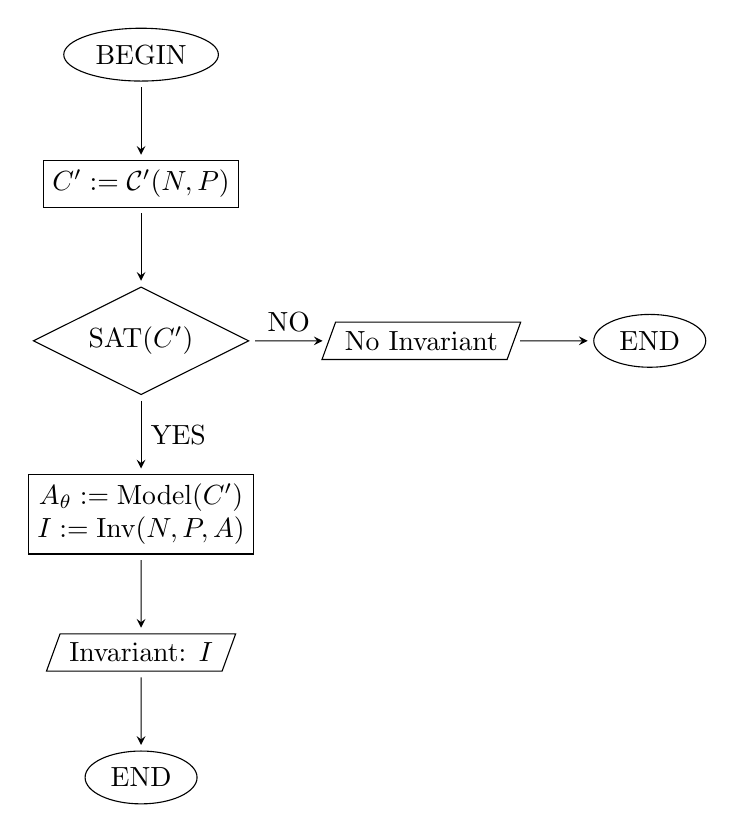
\begin{tikzpicture}
  \node[state] (begin) {BEGIN};
  \node[action, below=of begin] (c) {$C':=\mathcal C'(N, P)$};
  \node[decision, below=of c] (satc) {$\text{SAT}(C')$};
  \node[print, right=of satc] (noinv) {No Invariant};
  \node[action, below=of satc] (inv) {$A_\theta:=\text{Model}(C')$\\
                                  	$I := \text{Inv}(N, P, A)$};
  \node[print, below=of inv] (printinv) {Invariant: $I$};
  \node[state, right=of noinv] (end1) {END};
  \node[state, below=of printinv] (end2) {END};
 
  \draw (begin) edge (c);
  \draw (c) edge (satc);
  \draw (satc) edge node[above]{NO} (noinv);
  \draw (satc) edge node[right]{YES} (inv);
  \draw (noinv) edge (end1);
  \draw (inv) edge (printinv);
  \draw (printinv) edge (end2);
\end{tikzpicture}

\section{Method Safety by Refinement}

\paragraph{Example: Mutual exclusion algorithm in Delzanno2001}

\begin{verbatim}
* Code

bool m1 = false;
bool m2 = false;

// Thread 1:
while (true) {
  if (! m2 && ! test_and_set(m1)) {
    // critical section 1
    m1 = false
  }
  if (! m1 && ! test_and_set(m2)) {
    // critical section 2
    m2 = false
  }
}

// Thread 2:
while (true) {
  if (! m2 && ! test_and_set(m1)) {
    // critical section 1
    m1 = false
  }
  if (! m1 && ! test_and_set(m2)) {
    // critical section 2
    m2 = false
  }
}

Property: The number of threads in critical sections should be at most 1

* Petri net

Place m1 is marked in the net exactly if m1 is false in the algorithm.
Place m2 is marked in the net exactly if m2 is false in the algorithm.

\end{verbatim}

\paragraph{Example: Petri net for mutual exclusion algorithm in Delzanno2001}
\mbox{ } \\
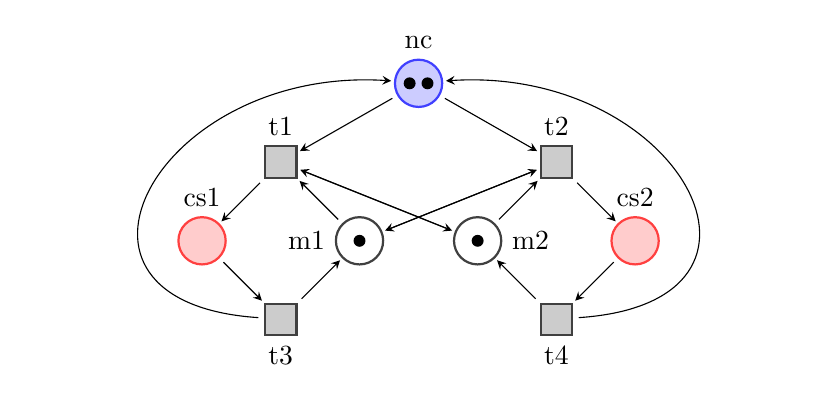
\begin{tikzpicture}[node distance=2cm]
  \node[blue place, tokens=2, label=above:nc] (nc) {};
  \node[place, tokens=1, label=right:m2, below of=nc, xshift=+0.75cm] (s2) {};
  \node[place, tokens=1, label=left:m1, below of=nc, xshift=-0.75cm] (s1) {};
  \node[red place, label=above:cs1, left of=s1] (cs1) {};
  \node[red place, label=above:cs2, right of=s2] (cs2) {};
  \node[transition, label=above:t1] (t1) at ($(s1)!0.5!(cs1) + (0,1cm)$) {}
	edge [pre] (nc)
	edge [pre] (s1)
	edge [pre] (s2)
	edge [post] (cs1)
	edge [post] (s2);
  \node[transition, label=above:t2] (t2) at ($(s2)!0.5!(cs2) + (0,1cm)$) {}
	edge [pre] (nc)
	edge [pre] (s2)
	edge [pre] (s1)
	edge [post] (cs2)
	edge [post] (s1);
  \node[transition, label=below:t3] (t3) at ($(s1)!0.5!(cs1) - (0,1cm)$) {}
	edge [pre] (cs1)
	edge [post] (s1)
	edge [post,bend left,min distance=3cm, out=115, in=115] (nc);
  \node[transition, label=below:t4] (t4) at ($(s2)!0.5!(cs2) - (0,1cm)$) {}
	edge [pre] (cs2)
	edge [post] (s2)
	edge [post,bend right,min distance=3cm, out=-115, in=-115] (nc);
\end{tikzpicture}
\begin{align*}
  P &= ( cs1 + cs2 \le 1 ) \\
  \neg P &= ( cs1 + cs2 \ge 2 )
\end{align*}

\paragraph{Intermediate results}
Constraints $\mathcal C(N)$ with
$M =\begin{pmatrix}nc & m1 & m2 & cs1 & cs2 \end{pmatrix}^T$,
$M_0 =\begin{pmatrix}2 & 1 & 1 & 0 & 0 \end{pmatrix}^T$,
$X =\begin{pmatrix}t1 & t2 & t3 & t4 \end{pmatrix}^T$ and
$C =\begin{pmatrix}
  -1 & -1 & 1 & 1 \\
  -1 &  0 & 1 & 0 \\
   0 & -1 & 0 & 1 \\
  1 & 0 & -1 & 0 \\
  0 & 1 & 0 & -1
\end{pmatrix}$:
\begin{align*}
  nc   =& 2 - t1 - t2 + t3 + t4 \\
  m1  =& 1 - t1 + t3 \\
  m2  =& 1 - t2 + t4 \\
  cs1 =& 0 + t1 - t3 \\
  cs2 =& 0 + t2 - t4 \\
  nc \ge& 0 \\
  m1 \ge& 0 \\
  m2 \ge& 0 \\
  cs1 \ge& 0 \\
  cs2 \ge& 0
\end{align*}

Satisfying assignment is
$M =\begin{pmatrix}0 & 0 & 0 & 1 & 1 \end{pmatrix}^T$ and
$X =\begin{pmatrix}1 & 1 & 0 & 0 \end{pmatrix}^T$.

A set satisfying the trap conditions is $S = \{m1, m2\}$.

The trap constraint is $\delta = (m1 + m2 \ge 1)$.

With the additional constraint, the set of constraints is unsatisfiable.

\paragraph{Technique trap conditions} For a petri net $N$ and an assignment $A$,
find a set $S$ that satisfies
\begin{enumerate}
  \item $S$ is a trap in the net $N$.
  \item $S$ is marked in the initial marking $M_0$.
  \item $S$ is unmarked in the assignment $A$.
\end{enumerate}
For such a set $S$, generate a constraint
$\delta = \left( \sum_{s \in S} s \ge 1 \right)$, ensuring the
trap is marked in any assignment.

\paragraph{Method Safety by Refinement}
\mbox{ } \\
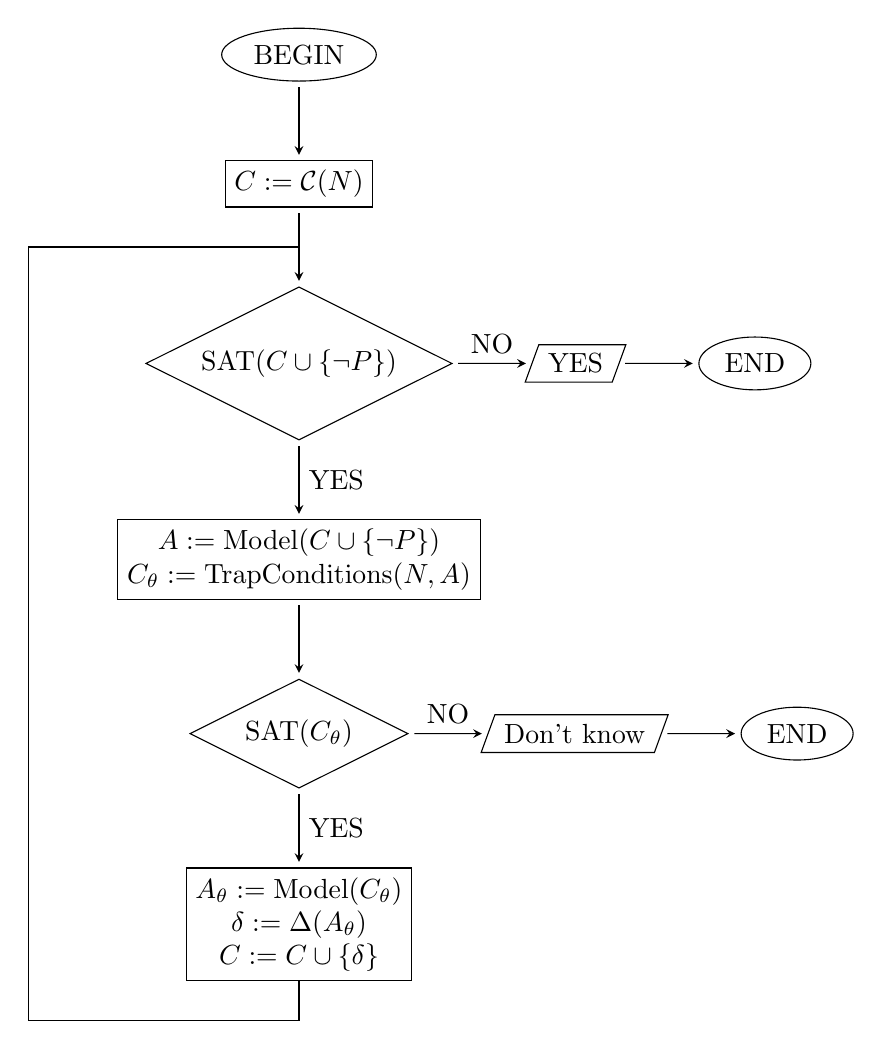
\begin{tikzpicture}
  \node[state] (begin) {BEGIN};
  \node[action, below=of begin] (c) {$C:=\mathcal C(N)$};
  \node[decision, below=of c] (satc) {$\text{SAT}(C \cup \{\neg P\})$};
  \node[action, below=of satc] (modelc) {$A:=\text{Model}(C \cup \{\neg P\})$\\
                               	$C_{\theta}:=\text{TrapConditions}(N, A)$};
  \node[decision, below=of modelc] (satctheta) {$\text{SAT}(C_\theta)$};
  \node[action, below=of satctheta] (modelctheta) {$A_\theta:=\text{Model}(C_\theta)$\\
                                    	$\delta:=\Delta(A_\theta)$\\
                                    	$C:=C \cup \{\delta\}$};
  \node[print, right=of satc] (yes) {YES};
  \node[print, right=of satctheta] (dontknow) {Don't know};
  \node[state, right=of yes] (end1) {END};
  \node[state, right=of dontknow] (end2) {END};

  \draw (begin) edge (c);
  \draw (c) edge coordinate[pos=.5] (edgein) (satc);
  \draw (satc) edge node[above]{NO} (yes);
  \draw (yes) edge (end1);
  \draw (satc) edge node[right]{YES} (modelc);
  \draw (modelc) edge (satctheta);
  \draw (satctheta) edge node[above]{NO} (dontknow);
  \draw (dontknow) edge (end2);
  \draw (satctheta) edge node[right]{YES} (modelctheta);
  \draw (modelctheta.south) -- ([yshift=-0.5cm] modelctheta.south)
  -| ([xshift=-2cm] modelctheta.west) |- (edgein);
\end{tikzpicture}

\section{Method Invariant by Refinement}

\paragraph{Example}
See example for method Safety by Refinement.

\paragraph{Intermediate results}
Constraints $\mathcal C'(N)$ with
$Y_1 = \begin{pmatrix}target1 \end{pmatrix}$,
$Y_2 = \begin{pmatrix}trap2 \end{pmatrix}$,
$Y_3 =\begin{pmatrix}nc & m & cs1 & cs2\end{pmatrix}$,
the trap from the trap refinement as
$D =\begin{pmatrix}0 & 1 & 1 & 0 & 0 \end{pmatrix}$,
$A =\begin{pmatrix}0 & 0 & 0 & 1 & 1 \end{pmatrix}$ and
$b =\begin{pmatrix}1 \end{pmatrix}$:

\begin{align*}
  target1 - trap1 - nc - m1 + cs1 \le& 0 \\ 
  target1 - trap1 - nc - m2 + cs2 \le& 0 \\ 
  - target1 + trap1 + nc + m1 - cs1 \le& 0 \\ 
  - target1 + trap1 + nc + m2 - cs2 \le& 0 \\ 
2 \cdot trap1 + 2 \cdot nc + m1 + m2 <& 2 \cdot target1 + trap1 \\
  target1 \ge& 0 \\
  trap1 \ge& 0 \\
  nc \ge& 0 \\
  m1 \ge& 0 \\
  m2 \ge& 0 \\
  cs1 \ge& 0 \\
  cs2 \ge& 0
\end{align*}

Satisfying assignment is
$Y_1 = \begin{pmatrix} 1 \end{pmatrix}$,
$Y_2 = \begin{pmatrix} 1 \end{pmatrix}$ and
$Y_3 = \begin{pmatrix}0 & 0 & 0 & 0 & 0 \end{pmatrix}$.

Invariant $\text{Inv}(N, D, P, A) =
((cs1 + cs2 + m1 + m2 \le 2) \land (m1 + m2 \ge 1))$.

\paragraph{Technique}
\begin{align*}
  \mathcal C'(N, D, P) =& ( ( ( Y_1 \cdot A + Y_2 \cdot D + Y_3) \cdot C \le 0) \land \\
& ((Y_1 \cdot A + Y_2 \cdot D + Y_3) \cdot M_0 < Y_1 \cdot b + Y_2 \cdot \mathbf{1}) \land \\
& (Y_1 \ge 0) \land (Y_2 \ge 0) \land (Y_3 \ge 0)) \\
  \text{Inv}(N, D, P, A) =& ( ( Y_1 \cdot A + Y_2 \cdot D + Y_3) \cdot M \le ( Y_1 \cdot A + Y_2 \cdot D + Y_3) \cdot M_0) \land ( D \cdot M \ge \mathbf{1} )
\end{align*}
where $M_0$ is the initial marking, $C$ is the incidence matrix of the net, $A\cdot M \ge b$ is equivalent to $\neg P$ and $D \cdot M \ge \mathbf{1}$ is equivalent to the trap constraints.

\paragraph{Method Invariant by Refinement}
\mbox{ } \\
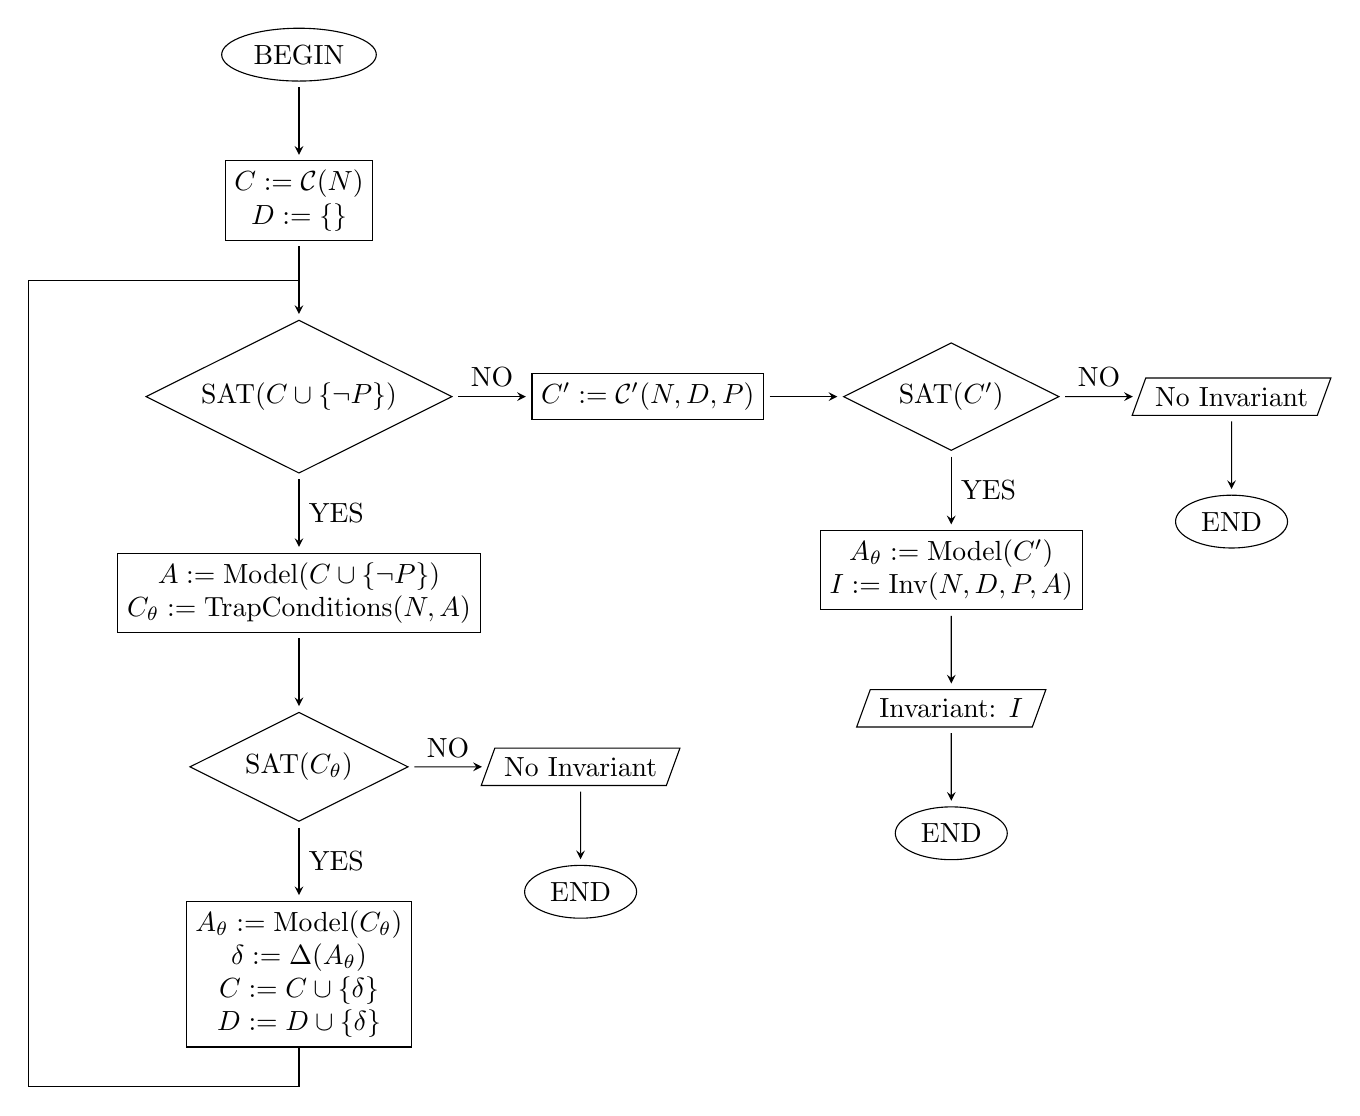
\begin{tikzpicture}
  \node[state] (begin) {BEGIN};
  \node[action, below=of begin] (c) {$C:=\mathcal C(N)$\\
                                 	$D:=\{\}$};
  \node[decision, below=of c] (satc) {$\text{SAT}(C \cup \{\neg P\})$};
  \node[action, below=of satc] (modelc) {$A:=\text{Model}(C \cup \{\neg P\})$\\
                                   	$C_{\theta}:=\text{TrapConditions}(N, A)$};
  \node[decision, below=of modelc] (satctheta) {$\text{SAT}(C_\theta)$};
  \node[action, below=of satctheta] (modelctheta) {$A_\theta:=\text{Model}(C_\theta)$\\
                                        	$\delta:=\Delta(A_\theta)$\\
                                        	$C:=C \cup \{\delta\}$\\
                                        	$D:=D \cup \{\delta\}$};
  \node[print, right=of satctheta] (noinv2) {No Invariant};
  \node[state, below=of noinv2] (end3) {END};
   
  \node[action, right=of satc] (cprime) {$C':=\mathcal C'(N, D, P)$};
  \node[decision, right=of cprime] (satcprime) {$\text{SAT}(C')$};
  \node[action, below=of satcprime] (inv) {$A_\theta:=\text{Model}(C')$\\
                                      	$I := \text{Inv}(N, D, P, A)$};
  \node[print, below=of inv] (printinv) {Invariant: $I$};
  \node[print, right=of satcprime] (noinv) {No Invariant};
  \node[state, below=of noinv] (end1) {END};
  \node[state, below=of printinv] (end2) {END};
 
  \draw (cprime) edge (satcprime);
  \draw (satcprime) edge node[above]{NO} (noinv);
  \draw (satcprime) edge node[right]{YES} (inv);
  \draw (inv) edge (printinv);
  \draw (noinv) edge (end1);
  \draw (printinv) edge (end2);
 
  \draw (begin) edge (c);
  \draw (c) edge coordinate[pos=.5] (edgein) (satc);
  \draw (satc) edge node[above]{NO} (cprime);
  \draw (satc) edge node[right]{YES} (modelc);
  \draw (modelc) edge (satctheta);
  \draw (satctheta) edge node[above]{NO} (noinv2);
  \draw (noinv2) edge (end3);
  \draw (satctheta) edge node[right]{YES} (modelctheta);
  \draw (modelctheta.south) -- ([yshift=-0.5cm] modelctheta.south)
  -| ([xshift=-2cm] modelctheta.west) |- (edgein);
\end{tikzpicture}

\fi

\end{document}
